Najszerzej znanymi elementami fotonicznymi, które charakteryzują się jednokierunkową transmisją światła są izolatory Faradaya.  Podstawą ich działania jest zjawisko Faradaya, polegające na obrocie płaszczyzny polaryzacji światła przechodzącego przez ośrodek magnetooptyczny w~obecności zewnętrznego pola magnetycznego. W~tej pracy będziemy się zajmować możliwością uzyskania asymetrycznej transmisji w strukturach złożonych z~metalowych siatek, w~których nie występuje zjawisko magneto-optyczne, ani zjawiska nieniowe. Na podstawie tw.~o~wzajemności Lorentza można wykazać, że takie układy nie mogą być izolatorami rozumianymi w~takim sensie, że jeśli opiszemy je używając macierzy rozpraszania do opisu zależności między wejściami i wyjściami układu, zawsze otrzymamy macierz symetryczną~\cite{4171512}. Jednocześnie okazuje się, że twierdzenie to nie stoi to w sprzeczności z możliwością blokowania transmisji światła dla padania z jednej strony siatki i przepuszczania światła przy przeciwnym kierunku padania~\cite{lockyear2006one}.

W dalszej części tego rozdziału omawiane są podwójne metalowe siatki dyfrakcyjne~(ang. DMG - double metallic grating)\nomenclature{DMG}{ang. Double Metallic Grating - podwójna metalowa siatka dyfrakcyjna}. Dla rozróżnienia, w~odniesieniu do wcześniej omawianych siatek wykorzystywany jest termin SMG~(ang. single metallic grating).

\begin{figure}[tb]
	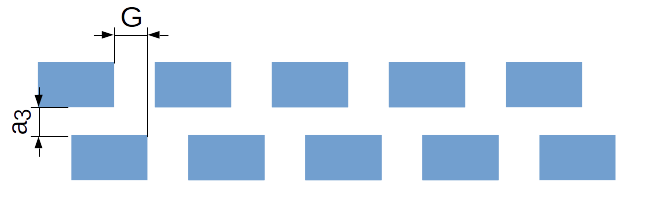
\includegraphics[width=\textwidth]{images/dmg/dmg_general_schem.png}
	\caption{Schematyczny obraz siatki DMG analizowanej w~pracy~\cite{cheng2007controllable}}
	\label{fig:cheng_dmg_schem}
\end{figure}

Przykład struktury typu DMG zbudowanej z~dwu siatek dyfrakcyjnych o~tym samym współczynniku wypełnienia i~okresie przedstawia rysunek~\ref{fig:cheng_dmg_schem}. Propozycję tego typu struktury jako uogólnienia SMG podał Chen Cheng i~inni~\cite{cheng2007controllable}, prezentując możliwość regulacji położenia maksimum widma transmisji przez dobór względnego usytuowania siatek. Zgodnie ze schematem na rysunku \ref{fig:cheng_dmg_schem} rozsunięcie siatek opisywane jest dwoma parametrami $G$ i~$a_3$. Możliwe jest uzyskanie niskiej transmisji przez strukturę dla szerokiego zakresu widmowego przy odpowiednim doborze względnego położenia siatek, co może zostać wykorzystane do budowy urządzeń mikromechanicznych kontrolujących współczynnik transmisji wiązki~\cite{cheng2007controllable}.

Analizę fizycznych mechanizmów prowadzących do nadzwyczajnej transmisji przez DMG zaczniemy od przypadku $a_3=0$ i~$G=0$. W takiej sytuacji uzyskujemy strukturę SMG o~grubości dwóch siatek składających się na DMG. Zgodnie z~wykresami na rysunku~\ref{fig:rezo-siat-H} dla tego typu siatki złożonej z~dwóch SMG o~grubości $h=300$~$\mu$m (por. rys. \ref{fig:schem-podklad-falo}) uzyskalibyśmy rezonanse transmisji takie jak dla siatki o~$h=600$~$\mu$m, czyli dla długości fali $\lambda \approx 400$~$\mu$m~i~$\lambda \approx 600$~$\mu$m. W wyniku stopniowego zwiększania odległości $a_3$ obserwujemy zbliżanie obu maksimów transmisji~\cite{cheng2008physical}. W odległość $a_3 \approx \frac{h}{2}$, następuje degeneracja obu modów, a maksimum transmisji występuje w~okolicach maksimów transmisji obu siatek SMG dla $\lambda \approx 560$~$\mu$m \cite{cheng2008physical}. Dalsze zwiększanie odległości powoduje znaczący spadek transmisji w~szerokim zakresie widma długości fali. Związane jest to ze słabym sprzężeniem stojącej fali powierzchniowej za pierwszą siatką SMG z~modami falowodów w~drugiej siatce SMG. Znaczne zwiększenie $a_3$, aż do odległości odpowiadającej warunkowi konstruktywnej interferencji w~rezonatorze Fabry-Perot tworzonego przez powietrze i~dwie warstwy o~efektywnych współczynnikach i~grubościach obliczonych zgodnie z~modelem efektywnym przedstawionym w~pracy \cite{shen2005mechanism} prowadzi do powstania kolejnych maksimów transmisji przez cały układ.

Niezależnie od modyfikowania własności transmisyjnych za pomocą odległości $a_3$ między siatkami SMG, przesunięcie maksimum transmisji jak i~jej blokowanie, można uzyskać zmieniając boczne przesunięcie siatek - $G$. Maksimum transmisji przez DMG można uzyskać również dla układu, w~którym $G$ dobrano tak, aby wyeliminować bezpośredni prześwit przez strukturę. Dla DMG jak na rysunku~\ref{fig:cheng_dmg_schem}, maksimum transmisji przez strukturę występuje dla $G$ równego zero lub połowie okresu SMG. Minimum transmisji napotykamy natomiast dla $G$ równego ćwierć okresu SMG~\cite{chan2006optical}.

\begin{figure}[tb]
	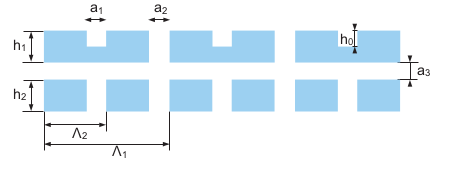
\includegraphics[width=\textwidth]{images/thz/1D-DMG-schemat.png}
	\caption{Schemat podwójnej siatki metalowej DMG zaprojektowanej do uzyskania transmisji asymetrycznej}
	\label{fig:1ddmg-schem}
\end{figure}


Możliwość zastosowania podwójnych siatek metalowych w~celu uzyskania różnej transmisji w~przypadku propagacji światła w~przeciwnych kierunkach przez strukturę zostało zaproponowane przez Ji Xu i~innych \cite{xu2011unidirectional}. W przeciwieństwie do wcześniejszych prac na temat DMG~\cite{cheng2007controllable,cheng2008physical,chan2006optical} w~zaproponowanej strukturze jedna z~siatek miała okres większy od długości fali dla której projektowano układ ($\Lambda>\lambda$). Autorzy błędnie interpretując wyniki symulacji FDTD twierdzili, że możliwe jest zastosowanie tego typu struktury jako elementu toru optycznego o~jednokierunkowej transmisji światła. Późniejsza wykonana przez nas analiza numeryczna i~eksperymentalna wykazała, że układ spełnia twierdzenie Lorenza o~wzajemności - w~związku z~czym nie może być  traktowany jako izolator optyczny \cite{jalas2013and}. Zwiększenie okresu jednej z~siatek umożliwiło zastosowanie rowków w~siatce wejściowej dla kierunku charakteryzującego się wysokim współczynnikiem transmisji~\cite{xu2011unidirectional}.

Odpowiednio dobrane parametry siatki podwójnej mogą prowadzić jednak do transmisji asymetrycznej. Różnica w~transmisji przejawia się niskim współczynnikiem transmisji przy oświetleniu prostopadłym jednej ze stron i~wysokim przy oświetleniu z~drugiej. Nie jest to jednak warunek wystarczający na realizację izolatora optycznego \cite{jalas2013and}, ponieważ w~przypadku wysokiej transmisji promieniowanie E-M jest uginane przez siatkę dyfrakcyjną. 

\begin{figure}[tb]
	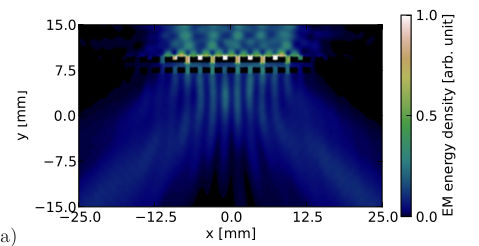
\includegraphics[width=\textwidth]{images/thz/opt_lett_gora.png}
	\caption{Rozkład gęstości energii pola E-M w~przypadku prostopadłego oświetlenia układu DMG zaprojektowanego do transmisji asymetrycznej od strony siatki z~rowkami~\cite{Stolarek:13}}
	\label{fig:trans_gora}
\end{figure}

\begin{figure}[tb]
	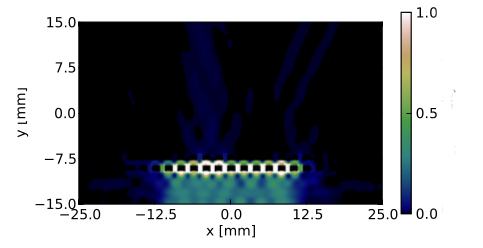
\includegraphics[width=\textwidth]{images/thz/opt_letters_dol.png}
	\caption{Rozkład gęstości energii pola E-M w~przypadku prostopadłego oświetlenia układu DMG zaprojektowanego do transmisji asymetrycznej od strony siatki podfalowej~\cite{Stolarek:13} }
	\label{fig:trans_dol}
\end{figure}

Fakt ten wynika z~budowy podwójnej siatki metalowej służącej do uzyskania transmisji asymetrycznej, która została przedstawiona na rysunku \ref{fig:1ddmg-schem}. Uzyskanie transmisji jednokierunkowej możliwe jest przy dobraniu parametrów układu tak, aby $\Lambda_1 = 2\Lambda_2$ oraz długość fali E-M $\lambda$ padającej na DMG  spełniała nierówność $\Lambda_2<\lambda<\Lambda_1$. Przywołując klasyczne prawo Braggów
\begin{equation}
	\Lambda \cdot \textrm{sin}(\alpha_k) = k \lambda,
\end{equation}
gdzie $\Lambda$ oznacza okres siatki dyfrakcyjnej, $k$ jest liczbą całkowitą numerującą rząd dyfrakcyjny padający pod kątem $\alpha_k$, a $\lambda$ długością padającej płaskiej fali E-M. Dla padania pod kątem $0^{\circ}$, zakładając otoczenie w~postaci powietrza z~obu stron DMG możemy wyprowadzić warunek na liczbę rzędów ugięcia uzyskiwanych przy użyciu siatki dyfrakcyjnej o~okresie $\Lambda$. 
\begin{equation}
	 0 \le |k| \le \frac { \Lambda }{\lambda},
\end{equation}
z którego wynika, że omawiany układ może wykazywać jednie -1,~0~i~+1 rząd ugięcia dla  $\Lambda=\Lambda_1$. Ze względu na podfalowy okres $\Lambda_2$ fala E-M padająca pod kątem $0^{\circ}$ będzie przez tę siatkę propagować się bez zmiany kierunku.  W wyniku interferencji za siatką dyfrakcyjną o~okresie $\Lambda_1$ możliwe jest wyeliminowanie jednego z~rzędów dyfrakcyjnych. Przedstawiona siatka projektowana jest dla długości fali $\lambda \approx 2.9$~mm, dla której kąt ugięcia $-1$~i~$+1$ rzędu wynosi $\alpha_{\pm 1} = 45^{\circ}$, która charakteryzuje się wygaszeniem rzędu zerowego. Wynik symulacji FDTD przedstawiający rozkład energii pola E-M w~przypadku oświetlenia struktury od strony siatki o~okresie $\Lambda_1$ przedstawia rysunek \ref{fig:trans_gora}.

\begin{SCfigure}
	\centering
	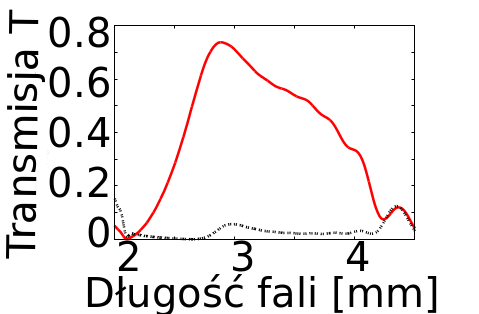
\includegraphics[width=0.5\textwidth]{images/thz/opt_lett_spect.png}
	\caption{Zależność współczynnika transmisji przez omawianą strukturę DMG od długości fali dla oświetlenia z~różnych stron. Wykres odpowiada DMG o~$\Lambda_1= 2 \Lambda_2 = 4.2$~mm, $a_1=a_2=a_3=0.7$~mm, $h_1=h_2=2 h_0=1$~mm~\cite{Stolarek:13}.}
	\label{fig:trans_freq}
\end{SCfigure}

 W innym ujęciu, strukturę typu DMG można analizować jako układ falowodów metal-dielektryk-metal, o~rozmiarach podfalowych ( $a_1,a_2,a_3 < \lambda$), dlatego wzbudzany może być w~nich jedynie mod podstawowy w~polaryzacji TM. Promieniowanie o~polaryzacji TE jest w~pełni odbijane przez omawiany układ. Dla $h_1=h_0$ i $a_3 \to 0$ struktura przypomina siatkę omawianą w~podrozdziale \ref{subart:rezo-grating} przedstawioną na rysunku \ref{fig:rezo-siat-H}. W przypadku $a_3 \ne 0$ możliwe jest dodatkowe sprzęganie pomiędzy falowodami poprzez falowód powstający pomiędzy siatkami dyfrakcyjnymi. Różnica w~fazie składowych pola E-M dochodzącego do otworów w~siatce o~okresie $\Lambda_1$ w~przypadku oświetlenia prostopadłego od strony siatki o~okresie $\Lambda_2$ w~omawianym przypadku wynosi $\pi$, w~wyniku czego współczynnik transmisji dla takiej sytuacji zbliża się do~0. Rozkład gęstości energii odpowiadający oświetleniu układu od strony siatki o~okresie $\Lambda_2$ przedstawia rysunek \ref{fig:trans_dol}.

W wyniku optymalizacji numerycznej parametrów struktury, prowadzonej za pomocą serii symulacji metodą FDTD, w~których parametry struktury podlegały ewolucji na bazie algorytmu genetycznego, uzyskano dla szerokiego zakresu długości fali znaczącą różnicę współczynników transmisji dla oświetlenia z~różnych stron DMG~\cite{Stolarek:13}. Zależność współczynnika transmisji przez DMG w~przeciwnych kierunkach od długości fali przedstawia wykres na rysunku \ref{fig:trans_freq}. Dalsze symulacje numeryczne wykazały, że możliwa jest niezależna zmiana otworów w~obu siatkach bez utraty transmisji jednokierunkowej w~celu poprawy kontrastu standardowo wyrażanego wzorem
\begin{equation}
C=\frac{|T_1 - T_2|}{T_1+T_2},
\label{eq:contrast}
\end{equation}
gdzie przez $T_1$ i~$T_2$ oznaczono natężeniowe współczynniki transmisji przy oświetleniu DMG odpowiednio od strony siatki o~okresie $\Lambda_1$ i~$\Lambda_2$.

Dla pełnego zrozumienia znaczenia kontrastu wprowadźmy dodatkowe definicje:
\begin{equation}
	\begin{gathered}
	R=T_1-T_2, \\
	Q=\frac{T_1}{T_2}.
	\end{gathered}
	\label{eq:rq-def}
\end{equation}
Zakładając, że $T_1>T_2$ (z czego wynika, że $Q>1$), możemy zapisać wyrażenie z~mianownika wzoru (\ref{eq:contrast}) za pomocą wprowadzonych zmiennych $R$ i~$Q$:
\begin{equation}
	T_1+T_2=\frac{Q+1}{Q-1} \cdot R,
\end{equation}
co po podstawieniu do wzoru (\ref{eq:contrast}) wskazuje, że pomimo tego, że różnica transmisji $R$  znajduje się w~liczniku wyrażenia, to sam kontrast zależny jest jedynie od ilorazu transmisji w~przeciwnych kierunkach i~wyraża się wzorem:
\begin{equation}
	C=\frac{Q-1}{Q+1}
	\label{eq:contrast-Q}.
\end{equation}
Oznacza to, że oprócz kontrastu $C$, przy analizie transmisji należy posługiwać się także transmisją $T_1$ lub różnicą $R$~\cite{stolarek2013broadband}. Równoważnie można prowadzić optymalizację tego typu struktury wykorzystując do tego wprowadzone oznaczenia $R$ i~$Q$. Dla odróżnienia od poprzednich siatek, w~których otwory w~obu siatkach SMG były równe $a_2$, wprowadzono oznaczenia $d_1$ i~$d_2$ - dla otworów w~siatkach o~okresie odpowiednio $\Lambda_1$ i~$\Lambda_2$. Zależność wprowadzonych w~(\ref{eq:rq-def}) współczynników od długości fali i~rozmiarów otworów przedstawiają wykresy na rysunku \ref{fig:qr-od-d}.

\begin{figure}[tb]
	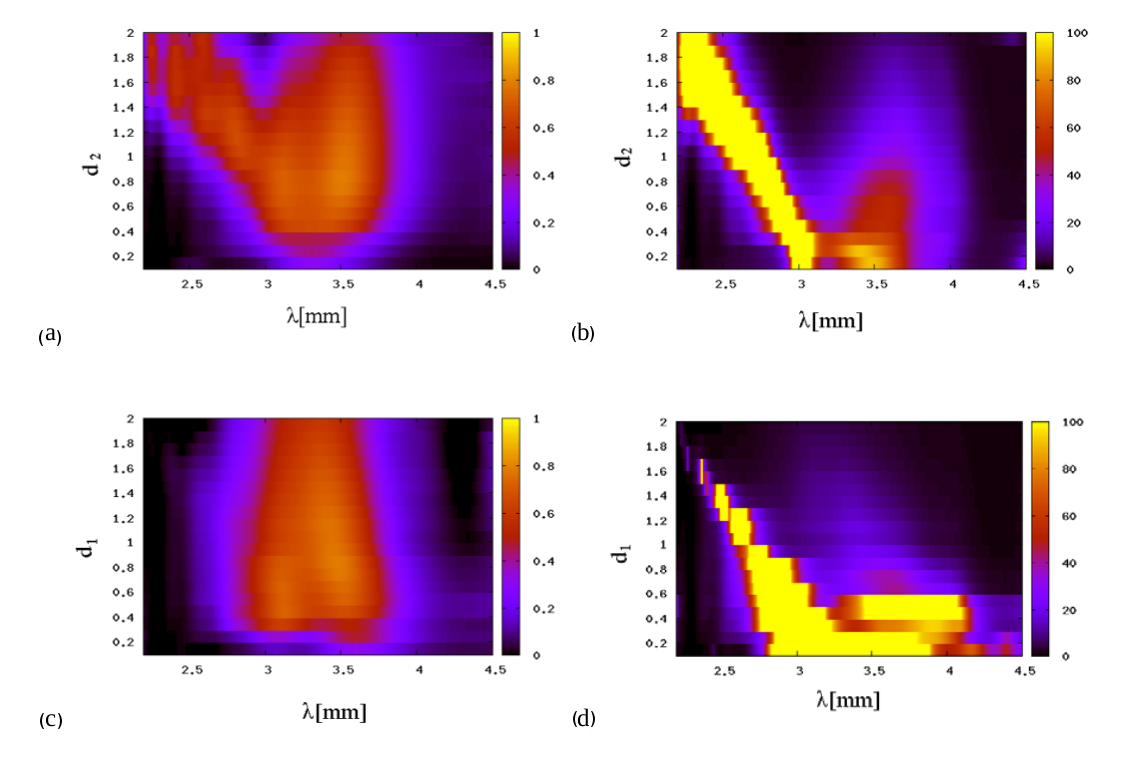
\includegraphics[width=\textwidth]{images/dmg/kontrast_maps.png}
	\caption{Zależność współczynników $R$ (a) i~(c), oraz $Q$ (b) i~(d) od długości fali $\lambda$ oraz od rozmiarów otworów w~obu siatkach. Rozmiar otworów dla (a) i~(b) jest   jest równy $d_1=0.7$~mm, natomiast dla (c) i~(d) $d_2=0.7$~mm }
	\label{fig:qr-od-d}
\end{figure}

Oczekiwane parametry pracy wielowarstwy to $R=1$ oraz $Q \to \infty$ oznaczające transmisję jednokierunkową. Na podstawie wyników zaprezentowanych na rysunku \ref{fig:qr-od-d} możemy stwierdzić, że optymalnymi rozmiarami otworów są $d_1\in(0.3,0.5)$~mm, oraz $d_2\in(0.6,1)$~mm w~przypadku pracy układu dla długości fali z~zakresu $\lambda \in (2.5, 4)$mm. Dodatkowo stwierdzić można, że
\begin{itemize}
	\item Zwiększanie $d_1$ powyżej wskazanego zakresu powoduje znaczne zwiększenie transmisji w~kierunku blokującym - co objawia się spadkiem kontrastu na wykresie \ref{fig:qr-od-d}d.
	\item Zmiana rozmiaru $d_2$ nie ma zasadniczego wpływu na $Q$, a tym samym na kontrast (\ref{eq:contrast-Q}), może jednak prowadzić do poszerzenia widma i~zwiększenia różnicy $R$ transmisji w~przeciwnych kierunkach (patrz rysunek \ref{fig:qr-od-d}a).
	\item Dla wąskiego zakresu długości fali w~okolicach $\lambda\approx2.6$~mm, możliwe jest uzyskanie wysokiego kontrastu $Q>100$ i~różnicy ${R\approx 0.7}$, dla ${d_1>1}$~mm. Taka struktura wykazuje jednak transmisję wynoszącą ok.~10\% dla fal dłuższych od $3$~mm~\cite{stolarek2013broadband}.
\end{itemize}
